\section{State Management}
\begin{frame}
    \frametitle{State Management}
    \begin{itemize}
        \item Jede Frontend Instanz des Editors inklusive des Backends führen den aktuellen Application State in einem eigenen Store.
        \item Dieser Store hält den Application State in zwei Instanzen der YJS Datenstruktur:
        \begin{description}
            \item[SyncedState] Wird im FE gerendert und im BE persistiert.
            \item[ShadowState] Wird mittels Aktionen(Messages / User Actions) manipuliert und dient zum Erstellen eines Diffs zum SyncedState.
        \end{itemize}
        \item Der Store bietet zwei Patch Methoden:
        \begin{description}
            \item[patchAsync] Aktualisiert beide States sofort und generiert periodisch Messages mit einem Patch.
            \item[patchSync] Aktualisiert im ersten Schritt den ShadowState, verschickt eine Message mit dem Patch und aktualisiert den SyncedState wenn der Patch verteilt wurde.
        \end{itemize}
        \item Aktionen die Konflikte generieren können, verwenden immer patchSync.
        \item Aktionen die möglichst rasch im FE angezeigt werden müssen und keine Konflikte generieren verwenden patchAsync.
    \end{itemize}
\end{frame}

\begin{frame}
    \frametitle{Store}
    \begin{itemize}
        \item Der Store verteilt jede State-Anpassung, je nach Änderung, sofort oder mit einem kleinen Delay über die Message Queue.
        \item Für alle Änderungen wird ein Diff erstellt und nur das Diff des States wird über die Message Queue verteilt.
        \item Beim Generieren dieser Diffs kommt YJS ins Spiel:
        \begin{itemize}
            \item YJS kann aus seiner Datenstruktur Patches generieren, welche kommutativ und idempotent angewendet werden können.
            \item Sollten Messages nicht in der korrekten Reihenfolge oder mehrfach ankommen haben alle Clients nach dem verteilen der Messages denselben Zustand.
            \item Die Message Queue garantiert eine excatly-once (QoS 2) Auslieferung aller Messages.
        \end{itemize}
    \end{itemize}
\end{frame}

\begin{frame}
    \frametitle{Patch Sync}
    So läuft ein synchrones Patch ab:
    \centering
    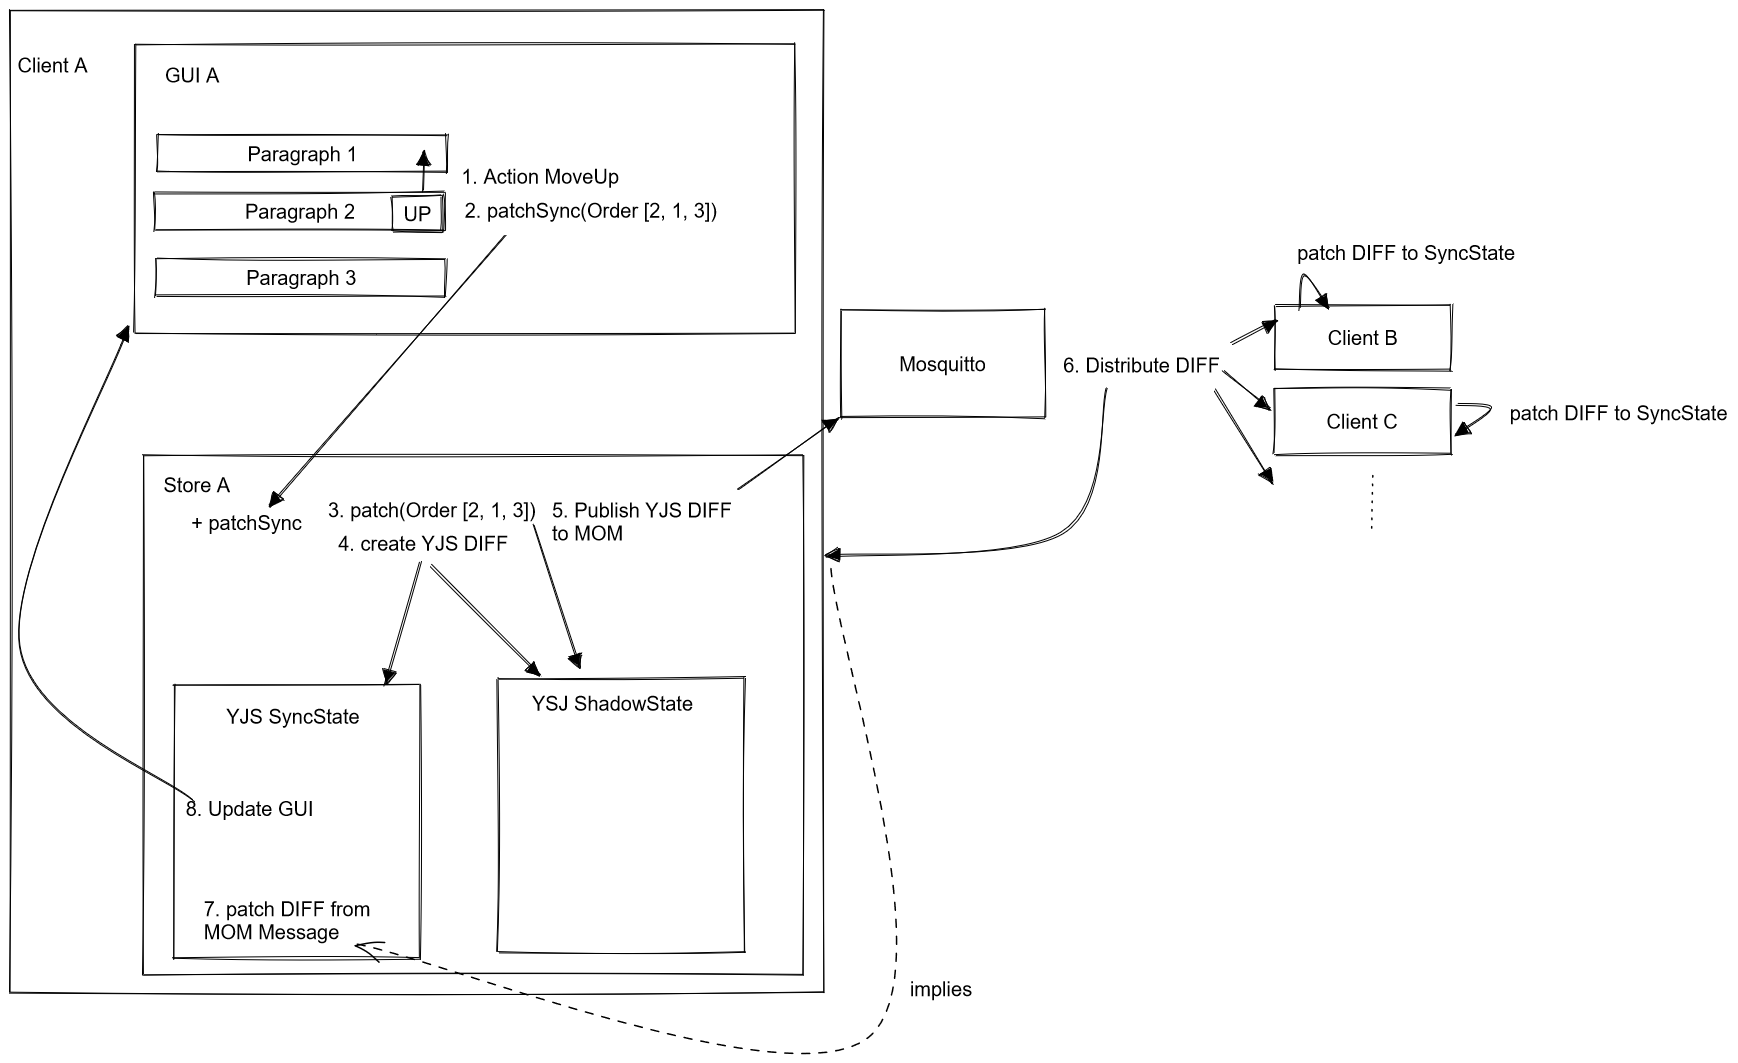
\includegraphics[height=6cm]{media/patchSync}\label{fig:Patch Sync Skizze}
\end{frame}

\begin{frame}
    \frametitle{Patch Async}
    So läuft ein asynchrones Patch ab:
    \centering
    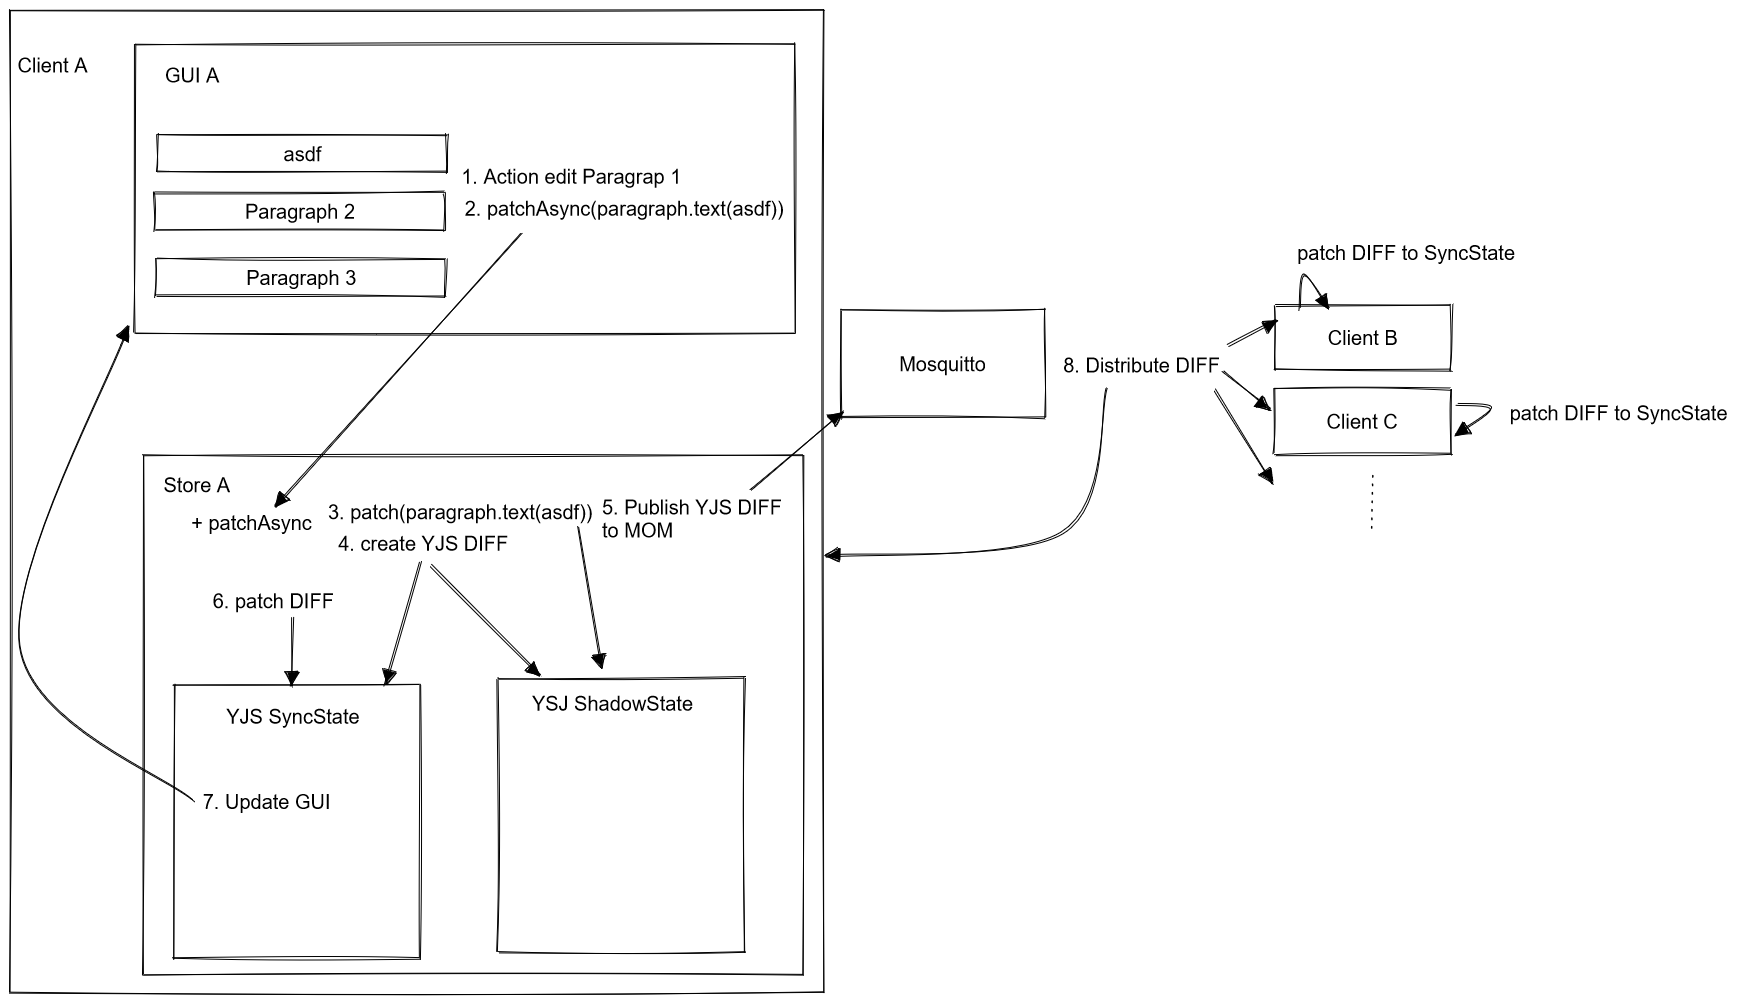
\includegraphics[height=6cm]{media/patchAsync}\label{fig:Patch Async Skizze}
\end{frame}

\begin{frame}
    \frametitle{Inhalt des Stores}
    Der Shared State wird in folgendem Format in der YJS Datenstruktur gespeichert:
    \lstinputlisting[language=json, basicstyle=\tiny]{media/sharedStore.json}
\end{frame}



